\documentclass[12pt, a4paper]{article}

% Required Packages
\usepackage[utf8]{inputenc}
\usepackage{graphicx} % For images (like the RVCE logo and project photos)
\usepackage[margin=1in]{geometry} % For page margins
\usepackage{amsmath, amssymb} % For mathematical symbols if needed
\usepackage{fancyhdr} % For custom headers/footers
\usepackage{enumitem} % For custom list environments
\usepackage{hyperref} % For clickable links (optional, but good for TOC)
\usepackage{float} % For better control over figure placement
\usepackage{xcolor} % For colors, if needed
\usepackage{listings} % For pseudocode
\usepackage{caption} % For customizing captions
\usepackage{booktabs} % For professional looking tables

% --- Customizing Header/Footer ---
\pagestyle{fancy}
\fancyhf{} % Clear all headers and footers
\rhead{EL Report} % Right header 
\lhead{CS344AI} % Left header 
\rfoot{\thepage} % Page number on the right footer
\renewcommand{\headrulewidth}{0.4pt} % Line under header
\renewcommand{\footrulewidth}{0pt} % No line under footer

% GEOMETRY
\geometry{
    a4paper,
    total={170mm,257mm},
    left=20mm,
    top=20mm,
}

% HYPERREF SETUP
\hypersetup{
    colorlinks=false,
    linkcolor=blue,
    filecolor=magenta,      
    urlcolor=cyan,
    pdftitle={City-Scale Optimal Path Finder},
    pdfpagemode=FullScreen,
    pdfborder={0 0 0}  
}

% LISTINGS (CODE) STYLE
\definecolor{codegreen}{rgb}{0,0.6,0}
\definecolor{codegray}{rgb}{0.5,0.5,0.5}
\definecolor{codepurple}{rgb}{0.58,0,0.82}
\definecolor{backcolour}{rgb}{0.95,0.95,0.92}

\lstdefinestyle{mystyle}{
    backgroundcolor=\color{backcolour},   
    commentstyle=\color{codegreen},
    keywordstyle=\color{magenta},
    numberstyle=\tiny\color{codegray},
    stringstyle=\color{codepurple},
    basicstyle=\ttfamily\footnotesize,
    breakatwhitespace=false,         
    breaklines=true,                 
    captionpos=b,                    
    keepspaces=true,                 
    numbers=left,                    
    numbersep=5pt,                  
    showspaces=false,                
    showstringspaces=false,
    showtabs=false,                  
    tabsize=2
}
\lstset{style=mystyle}

% --- Title Page Setup ---
\begin{document}

\clearpage
\tableofcontents
\clearpage

% --- Abstract ---
\section{Abstract} 
This report details the design and implementation of a Resilient Communication Framework for Disaster Scenarios using ESP32-based Opportunistic Mesh and Mobile Relay Systems. The primary goal is to establish a lightweight, infrastructure-free IoT system capable of transmitting emergency messages when conventional communication networks (internet, cellular, fixed mesh) are unavailable. The system employs ESP32 nodes equipped with sensors to detect disaster events, broadcasting SOS packets locally via ESP-NOW using a Time-to-Live (TTL) based flooding mechanism. For messages unable to reach a receiver within range, a mobile data mule model is integrated, where mobile ESP32 gateways (e.g., on UAVs or rescue vehicles) opportunistically collect and deliver stored messages to a central base station. This hybrid approach ensures message delivery resilience in critical, post-disaster environments.

% --- Introduction ---
\section{Introduction} 
Disaster scenarios, such as earthquakes, floods, or other natural calamities, frequently lead to the catastrophic failure of traditional communication infrastructure, including cellular networks, internet services, and fixed mesh systems. This loss of connectivity severely hampers rescue operations, information dissemination, and victim coordination, often leading to increased casualties and prolonged recovery efforts. Existing IoT solutions often rely on stable network infrastructure, which is precisely what becomes compromised during a disaster. There is a critical need for robust, autonomous communication systems that can operate independently of damaged infrastructure.

This project addresses this gap by proposing a resilient communication framework specifically designed for disaster-prone areas. It leverages the low-power and wireless capabilities of ESP32 microcontrollers to create an ad-hoc, self-forming network. The framework combines two key communication paradigms: a local opportunistic mesh using ESP-NOW for direct node-to-node communication and rebroadcasting, and a mobile relay (data mule) system for collecting and forwarding messages from isolated areas to a central base station. This hybrid strategy aims to maximize message delivery probability in dynamic and challenging environments, ensuring that critical emergency alerts and sensor data can reach responders even when the grid is down.

\subsection{Project Goal}
The goal of this project is to design a lightweight, infrastructure-free IoT system using ESP32 nodes that enables emergency message transmission even in the absence of internet, cellular, or fixed mesh infrastructure, combining local broadcast/rebroadcast and mobile data mule models.

\subsection{System Overview}
The system comprises ESP32-based devices deployed in a disaster-prone area. Each device is equipped with sensors such as GPS, accelerometers, and optional gas/smoke detectors. Upon detecting a disaster event or receiving a distress trigger, a device initiates the creation of an SOS packet. This packet is then broadcast locally using ESP-NOW with a Time-to-Live (TTL) mechanism for controlled flooding. If no receiver is within direct communication range, the message is stored locally on the device, awaiting collection by a mobile gateway. Mobile ESP32 gateways, integrated into entities like UAVs or rescue trucks, opportunistically collect these stored messages via proximity and subsequently deliver them to a base station or central receiver when in range.

\subsection{Network Roles}
The framework defines specific roles for the ESP32 devices within the network:
\begin{itemize}
    \item \textbf{Sender Node:} Senses events (e.g., earthquake, gas leak), creates an SOS packet, broadcasts it, and stores it locally for backup.
    \item \textbf{Passive Rebroadcaster:} Receives SOS packets, marks them as seen to avoid duplicates, and rebroadcasts them with a decremented TTL if TTL is greater than 0.
    \item \textbf{Mobile Gateway Node:} Scans for nearby sender nodes, collects stored messages via proximity, buffers them, and delivers all stored messages to a designated base station when in range. These can be deployed on UAVs or rescue trucks.
    \item \textbf{Receiver Node / Base Station:} The final destination for messages, responsible for reading, storing, and acting upon the received data.
\end{itemize}

\subsection{Message Packet Structure}
All communication within the network utilizes a standardized JSON-like message packet structure. This structure includes critical information for identification, localization, and event details:
\begin{lstlisting}[caption=SOS Message Packet Structure]
{
  "message_id": "auto-generated (MAC + timestamp)",
  "sender_mac": "MAC address of originating ESP32",
  "timestamp": "UTC or local time",
  "gps": { "lat": 12.935, "lon": 77.614 },
  "sensors": {
    "earthquake": true,
    "motion": 1.3,
    "gas_alert": false,
    "temperature": 34.2
  },
  "priority": "HIGH",
  "ttl": 3
}
\end{lstlisting}
Each node maintains a cache of `message\_id's it has already processed to prevent redundant rebroadcasting and optimize network traffic.

\subsection{Key Components}
The following hardware components are integral to the functionality of the ESP32-based system:
\begin{itemize}
    \item \textbf{ESP32:} The base microcontroller unit (MCU) is responsible for all logic and communication protocols. (Note: Project description mentions ESP8266 for pinout, but ESP32 is the primary MCU for the project concept.)
    \item \textbf{GPS Module (e.g., NEO-6M):} Provides location awareness for tagging distress messages with precise coordinates.
    \item \textbf{MPU6050 / ADXL345:} Accelerometer and gyroscope for earthquake detection by monitoring acceleration thresholds.
    \item \textbf{MQ-2 / MQ-135:} Gas/smoke detection sensors for identifying hazardous environmental conditions.
    \item \textbf{DHT22 or BMP280:} Temperature and humidity sensors for environmental monitoring and alerting on extreme conditions.
    \item \textbf{OLED Display (optional):} Provides visual feedback and status updates for field testing and debugging.
\end{itemize}

% --- Block Diagram and Description ---
\section{Block Diagram and Description} 
\subsection{Overall System Block Diagram}
\begin{figure}[htbp]
    \centering
    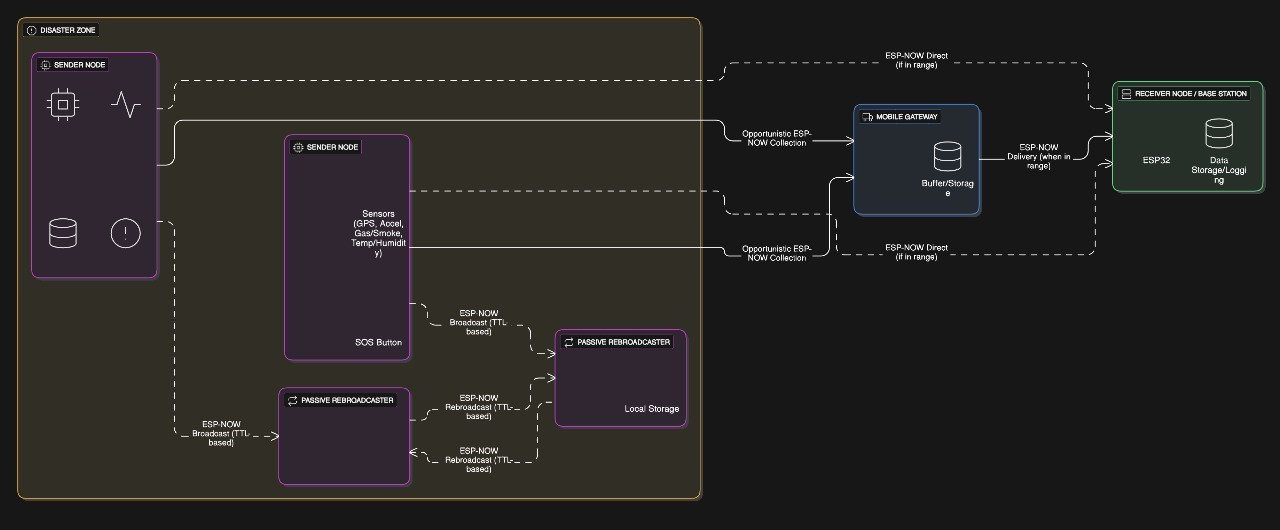
\includegraphics[width=0.9\textwidth]{image.jpg} % Placeholder for your system block diagram
    \caption{Overall System Block Diagram}
    \label{fig:system_block_diagram}
\end{figure}
\textit{Description:} The overall system block diagram illustrates the interaction between different types of nodes. Sender nodes (equipped with sensors and communication modules) detect events and initiate message broadcasting. Passive rebroadcasters extend the reach of these messages. Mobile gateways act as intermediate carriers, connecting isolated sender nodes to the central receiver/base station. All nodes leverage ESP-NOW for local communication and store messages for resilience.

\subsection{Individual Node Block Diagram}
\begin{figure}[htbp]
    \centering
    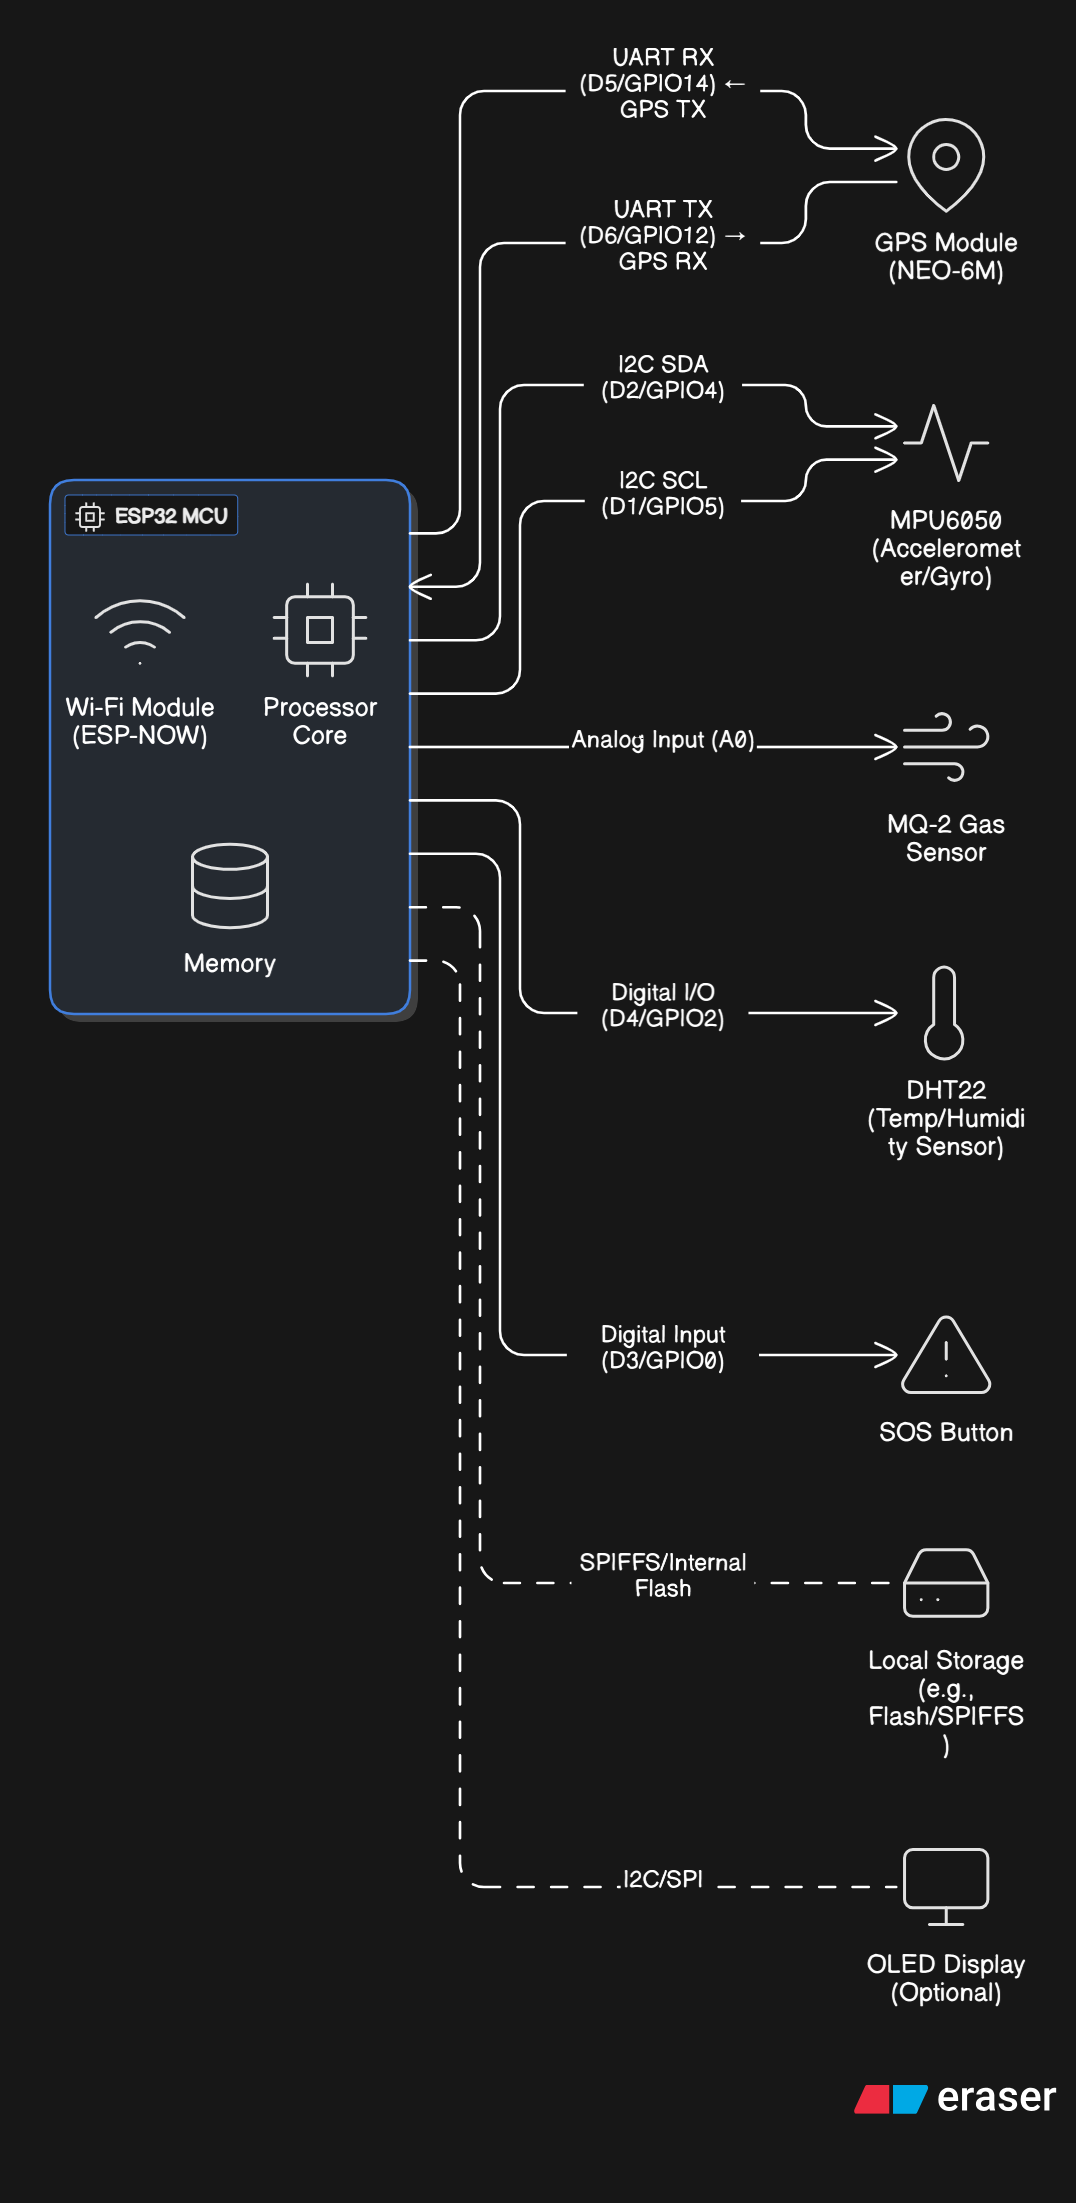
\includegraphics[width=0.7\textwidth]{image2.png} % Placeholder for your individual node block diagram
    \caption{Individual ESP32 Node Block Diagram}
    \label{fig:node_block_diagram}
\end{figure}
\textit{Description:} An individual ESP32 node typically comprises an ESP32 microcontroller as its core processing unit. It interfaces with various sensors (GPS, Accelerometer, Gas, Temperature/Humidity) to gather environmental data. A push button provides a manual SOS trigger. Communication is primarily handled by the ESP32's built-in Wi-Fi for ESP-NOW. Local storage (e.g., on flash memory or SD card) is crucial for buffering messages until they can be transmitted or collected by a mobile gateway. An optional OLED display provides local status information.

% --- IOT- 10 Design Steps ---
\section{IOT- 10 Design Steps} 
While a specific "10 design steps" methodology for IoT wasn't explicitly detailed in the project overview, we will integrate the project's implementation and design principles into a logical flow relevant to IoT development.

\subsection{1. Defining the Problem and Goal}
The problem is the lack of resilient communication in disaster scenarios due to infrastructure failure. The goal is to create an infrastructure-free IoT system using ESP32s for emergency message transmission via opportunistic mesh and mobile relays.

\subsection{2. Identifying Stakeholders and Use Cases}
\begin{itemize}
    \item \textbf{Stakeholders:} Victims in disaster zones, rescue teams, emergency services, government agencies.
    \item \textbf{Use Cases:}
        \begin{itemize}
            \item Automatic detection of earthquakes/gas leaks and sending SOS alerts.
            \item Manual distress signaling via a push button.
            \item Propagation of emergency messages through a localized mesh network.
            \item Collection of messages from isolated areas by mobile rescue units.
            \item Delivery of collected messages to a central command center.
        \end{itemize}
\end{itemize}

\subsection{3. Sensor Selection and Data Collection}
Based on the use cases, the following sensors are selected for data collection:
\begin{itemize}
    \item \textbf{GPS (NEO-6M):} For location tagging of SOS packets. Polled every 30 seconds.
    \item \textbf{MPU6050 (Accelerometer):} For earthquake detection by monitoring acceleration thresholds.
    \item \textbf{MQ-2/MQ-135 (Gas Sensor):} For gas leak detection, checking against calibrated baselines.
    \item \textbf{DHT22/BMP280 (Temperature/Humidity):} For environmental monitoring and alerting on extremes.
    \item \textbf{Push Button:} For manual SOS trigger via debounced interrupt.
\end{itemize}

\subsection{4. Connectivity and Communication Protocols}
The project leverages ESP32's Wi-Fi capabilities for communication:
\begin{itemize}
    \item \textbf{ESP-NOW:} Selected for short-range, connectionless communication, ideal for the opportunistic mesh (broadcast/rebroadcast) without requiring a router or infrastructure.
    \item \textbf{Ad-hoc / Opportunistic Mesh:} Achieved via TTL-based flooding using ESP-NOW for local message propagation.
    \item \textbf{Mobile Data Mule Model:} Utilizes proximity detection and ESP-NOW for opportunistic message collection by mobile gateways and subsequent delivery to a base station.
\end{itemize}

\subsection{5. Data Processing and Intelligence at the Edge}
Each ESP32 node performs local data processing:
\begin{itemize}
    \item Sensor data reading and thresholding (e.g., `detectEarthquake()`, `detectGasLeak()`).
    \item Creation of structured SOS packets with auto-generated message IDs, MAC addresses, timestamps, GPS, and sensor data.
    \item Duplicate message detection using a cached \texttt{message\_id} list to prevent redundant rebroadcasting.
\end{itemize}

\subsection{6. Cloud/Backend Integration (Base Station/Receiver)}
The "Receiver Node / Base Station" acts as the central hub for collected data. While not explicitly cloud-based in the project description, it serves a similar function by:
\begin{itemize}
    \item Receiving and logging messages from the mesh or mobile gateways.
    \item Storing received data for analysis or further action.
\end{itemize}
For a full IoT solution, this base station could connect to a cloud platform for data visualization, alert systems, and long-term storage.

\subsection{7. User Interface (Optional/Minimal)}
The project includes an optional OLED display for visual feedback during field testing. This serves as a local user interface to indicate device status or messages. For the base station, a simple console or web interface would be required to display received SOS messages.

\subsection{8. Security and Privacy (Considerations)}
While not detailed in the project overview, for a robust system, security considerations would include:
\begin{itemize}
    \item \textbf{Message Integrity:} Ensuring packets are not tampered with.
    \item \textbf{Authentication:} Verifying the legitimacy of sender nodes (though challenging in an infrastructure-less setup).
    \item \textbf{Anonymity (if required):} Depending on the use case, preserving sender anonymity might be a factor.
\end{itemize}
For this emergency system, priority is given to message delivery over strict security, but acknowledging these factors is crucial for future enhancements.

\subsection{9. Deployment and Management}
\begin{itemize}
    \item \textbf{Deployment:} ESP32 devices are deployed in disaster-prone areas. Mobile gateways are integrated into rescue vehicles/UAVs.
    \item \textbf{Management:} The system is designed to be self-organizing (opportunistic mesh) with minimal central management in the field. Firmware updates would need a manual or local-area provisioning mechanism.
\end{itemize}

\subsection{10. Business Model / Sustainability (Relevance to Project)}
The project focuses on a critical humanitarian need rather than a direct business model. Its sustainability lies in its ability to provide communication resilience during emergencies, potentially being adopted by disaster management agencies and NGOs. The low-cost nature of ESP32s contributes to its feasibility for widespread deployment.

% --- Implementation Details ---
\section{Implementation Details}
This section elaborates on the practical aspects of building the resilient communication framework.

\subsection{Communication Flow}
\subsubsection{Normal Flow:}
\begin{enumerate}
    \item A disaster event is detected, or an SOS button is pressed, leading to the creation of an SOS message packet.
    \item The packet is broadcast via ESP-NOW.
    \item Passive nodes in range receive the packet. If its \texttt{message\_id} has not been seen before, and \texttt{ttl > 0}, they decrement the \texttt{ttl} and rebroadcast the packet.
    \item The Receiver Node or Base Station ultimately receives and logs the message.
\end{enumerate}

\subsubsection{Backup Flow (Mobile Gateway):}
\begin{enumerate}
    \item Steps 1 and 2 from the normal flow occur.
    \item If no static receiver is in range, the sender node stores the message locally.
    \item A Mobile ESP32 unit (e.g., on a rescue drone) comes into proximity, triggering an auto-send of stored messages from the sender node to the mobile gateway.
    \item The mobile gateway buffers these messages.
    \item When the mobile gateway comes within range of the central receiver/base station, it sends all stored messages to it.
\end{enumerate}

\subsection{Pseudocode for Node Roles}
\subsubsection{Sender Node Pseudocode}
\begin{lstlisting}[language=C]
void setup() {
  initWiFi(); // Initialize ESP-NOW
  initSensors();
  initStorage(); // Initialize local storage (e.g., SPIFFS)
}

void loop() {
  // Check for disaster triggers
  if (detectEarthquake() || detectGasLeak() || isButtonPressed()) { // isButtonPressed includes debounce
    Packet msg = createSOSPacket();
    broadcast(msg); // Broadcast via ESP-NOW
    storeLocally(msg); // Store for mobile gateway backup
  }

  // Check if a mobile gateway is in range and send stored messages
  if (mobileGatewayDetected()) { // Requires a mechanism to detect gateway, e.g., scanning or beacon
    sendStoredMessagesToGateway();
  }
}
\end{lstlisting}

\subsubsection{Passive Rebroadcaster Pseudocode}
\begin{lstlisting}[language=C]
// ESP-NOW callback function for receiving messages
void onReceive(const Packet& msg) {
  if (!alreadySeen(msg.message_id)) { // Check if message ID is already in cache
    markSeen(msg.message_id); // Add to seen list
    if (msg.ttl > 0) {
      msg.ttl--; // Decrement Time-to-Live
      broadcast(msg); // Rebroadcast the packet
    }
  }
}
\end{lstlisting}

\subsubsection{Mobile Gateway Pseudocode}
\begin{lstlisting}[language=C]
void loop() {
  scanForNearbySenders(); // Continuously scan for sender nodes broadcasting messages
  if (msgReceived) { // If a message is received from a sender
    storeInBuffer(msg); // Store it temporarily
  }

  if (baseStationInRange()) { // If the base station is detected
    sendAllStoredMessagesToBase(); // Offload all collected messages
  }
}
\end{lstlisting}

\subsection{Sensor Integration and Pin Connections}
The following table summarizes the sensor integration and their respective pin connections on an ESP8266 NodeMCU, as specified in the project details. (Note: ESP32 pins might differ slightly, but the conceptual mapping is similar).

\begin{table}[H]
    \centering
    \caption{Sensor Pin Connections (ESP8266 NodeMCU)}
    \label{tab:sensor_pins}
    \begin{tabular}{llll}
        \toprule
        \textbf{Sensor / Module} & \textbf{Purpose} & \textbf{ESP8266 Label} & \textbf{GPIO Pin} \\
        \midrule
        DHT22 & Temp \& Humidity sensor & D4 & GPIO2 \\
        MPU6050 SDA & Motion detection (earthquakes) & D2 & GPIO4 \\
        MPU6050 SCL & Motion detection (earthquakes) & D1 & GPIO5 \\
        GPS RX (to GPS TX) & Location & D5 & GPIO14 \\
        GPS TX (to GPS RX) & Location & D6 & GPIO12 \\
        Gas Sensor (MQ-2/MQ-135) & Fire/gas alert & A0 & A0 (Analog Input) \\
        SOS Button & Emergency manual trigger & D3 & GPIO0 \\
        \bottomrule
    \end{tabular}
\end{table}

\subsubsection{Specific Implementation Notes for Sensors:}
\begin{itemize}
    \item \textbf{GPS (NEO-6M):} Polled every 30 seconds to cache the last known position. RX (GPS TX) connects to D5 (GPIO14), and TX (GPS RX) connects to D6 (GPIO12).
    \item \textbf{MPU6050:} Used for earthquake detection by monitoring acceleration thresholds. Requires `Wire.begin()` for I2C and `mpu.begin()` for initialization. Error handling is crucial.
    \item \textbf{MQ-2/MQ-135 Gas Sensor:} Connected to A0 (Analog Input). Its value (`analogRead(GAS\_SENSOR\_PIN)`) is compared against a defined threshold to determine a `gas\_alert`.
    \item \textbf{DHT22/BMP280:} For environmental monitoring, reading temperature and humidity every minute and triggering alerts on extremes.
    \item \textbf{Push Button:} Connected to D3 (GPIO0). Implemented with debounce logic to prevent false triggers (e.g., 300ms debounce time).
    \item \textbf{Power Management:} Interrupt-driven sensor monitoring is prioritized for power conservation, supported by a watchdog timer for reliability.
\end{itemize}

\subsection{Required Code Changes}
To ensure full functionality as per the design, the following modifications and checks are essential in the ESP32 firmware:
\begin{enumerate}
    \item \textbf{Enable Gas Sensor Input:}
    \begin{itemize}
        \item Uncomment or add \texttt{`\#define GAS\_SENSOR\_PIN A0'.}
        \item Read the analog value: \texttt{`int gasValue = analogRead(GAS\_SENSOR\_PIN);'.}
        \item Implement thresholding: \texttt{bool gas\_alert = gasValue > YOUR\_THRESHOLD;}.
        \item Ensure the `gas\_alert' field in the \texttt{`SOSPacket' structure is correctly populated.}
    \end{itemize}
    \item \textbf{MPU6050 Initialization and Error Handling:}
    \begin{itemize}
        \item Confirm `Wire.begin();` and `mpu.begin();` are called in `setup()`.
        \item Add error handling:
        \begin{lstlisting}[language=C]
if (!mpu.begin()) {
  Serial.println("Failed to find MPU6050 chip");
  while (1) { delay(10); } // Halt if MPU6050 not found
}
        \end{lstlisting}
    \end{itemize}
    \item \textbf{Sensor Data Usage in SOS Packet:}
    \begin{itemize}
        \item Verify that all sensor fields (\texttt{earthquake}, \texttt{motion}, \texttt{gas\_alert}, \texttt{temperature}) within the \texttt{SOSPacket} are correctly populated by their respective reading functions (e.g., \texttt{detectEarthquake()}, \texttt{getAccelerationMagnitude()}, \\
        \texttt{readGasSensor()}, \texttt{dht.readTemperature()}).
    \end{itemize}
    \item \textbf{Debounce the SOS Button:}
    \begin{itemize}
        \item Implement a debounced `isButtonPressed()` function for robust manual triggering:
        \begin{lstlisting}[language=C]
bool isButtonPressed() {
  static unsigned long lastDebounce = 0;
  if (digitalRead(SOS_BUTTON_PIN) == LOW && millis() - lastDebounce > 300) {
    lastDebounce = millis();
    return true;
  }
  return false;
}
        \end{lstlisting}
    \end{itemize}
\end{enumerate}

% --- Conclusion & Results ---
\section{Conclusion \& Results} 
This project successfully outlines a resilient communication framework for disaster scenarios, leveraging ESP32-based opportunistic mesh and mobile relay systems. The design addresses the critical challenge of communication loss during infrastructure failures by combining local broadcast/rebroadcast mechanisms with a store-and-forward mobile data mule approach. The detailed system overview, network roles, message structure, and component selection demonstrate a comprehensive understanding of the problem and a viable solution.

The implementation details, including pseudocode for various node roles and specific sensor integration with pin connections, provide a clear roadmap for developing the prototype. The proposed code changes highlight key areas for robust sensor handling and debouncing, crucial for reliable operation in an emergency context.

\subsection{Expected Results}
Upon successful implementation, the system is expected to demonstrate:
\begin{itemize}
    \item Reliable detection of disaster events (e.g., simulated earthquake, gas leak) by sensor-equipped nodes.
    \item Successful creation and local broadcasting of SOS packets via ESP-NOW.
    \item Effective rebroadcasting of messages by passive nodes, extending the communication range.
    \item Opportunistic collection of messages by mobile gateway nodes from isolated sender nodes.
    \item Successful delivery of all collected messages from mobile gateways to a central base station, even when direct static links are not available.
    \item Accurate tagging of SOS messages with GPS coordinates and sensor data.
    \item Minimal duplicate message propagation due to `message\_id' caching.
\end{itemize}

\subsection{Photos and Results}
\begin{figure}[H]
    \centering
    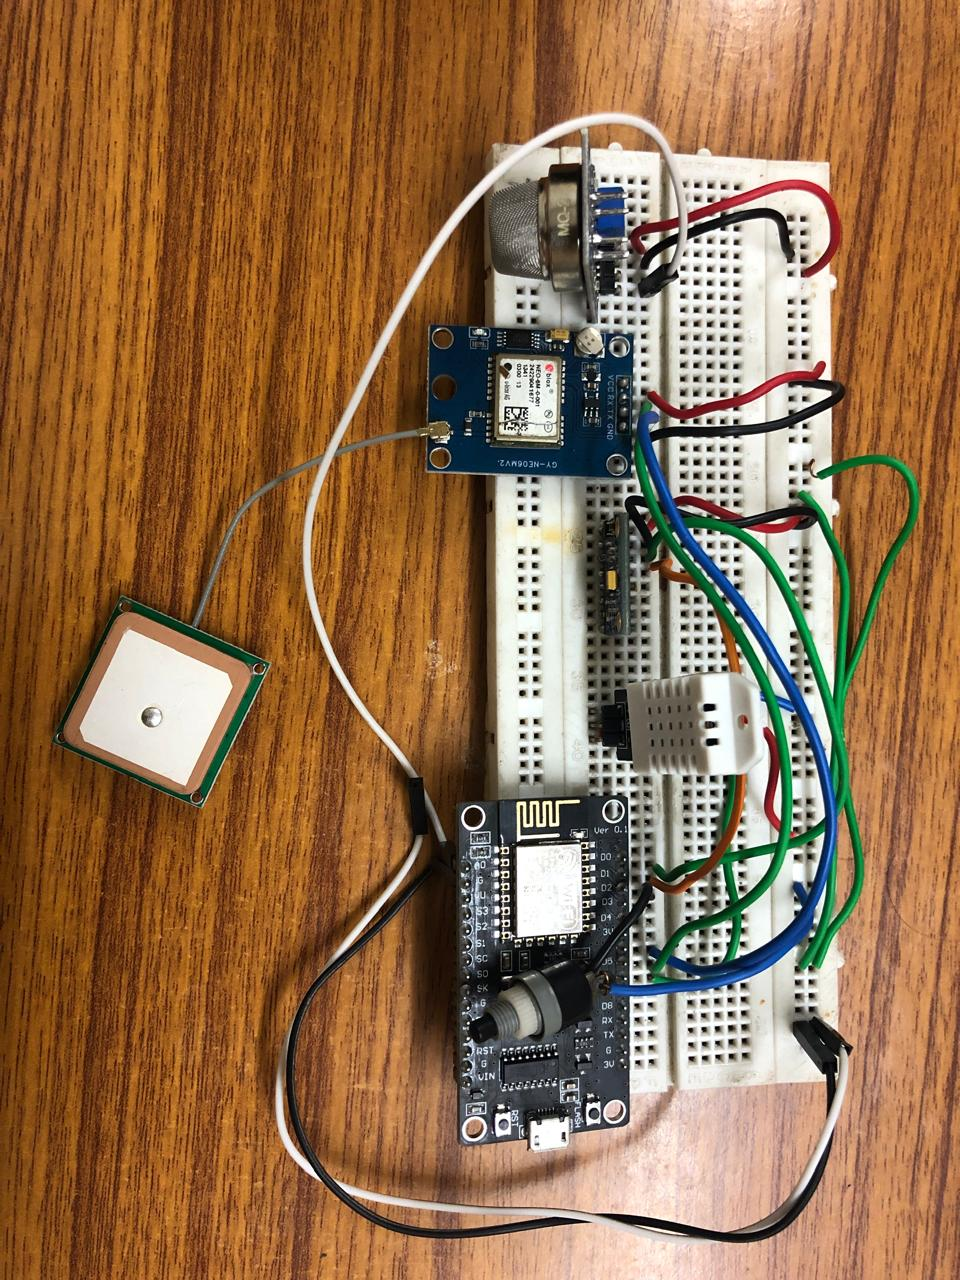
\includegraphics[width=0.8\textwidth]{prototype.jpg} % Placeholder for your prototype photo
    \caption{ESP32 Node Prototype with Sensors}
    \label{fig:prototype_1}
\end{figure}

\begin{figure}[H]
    \centering
    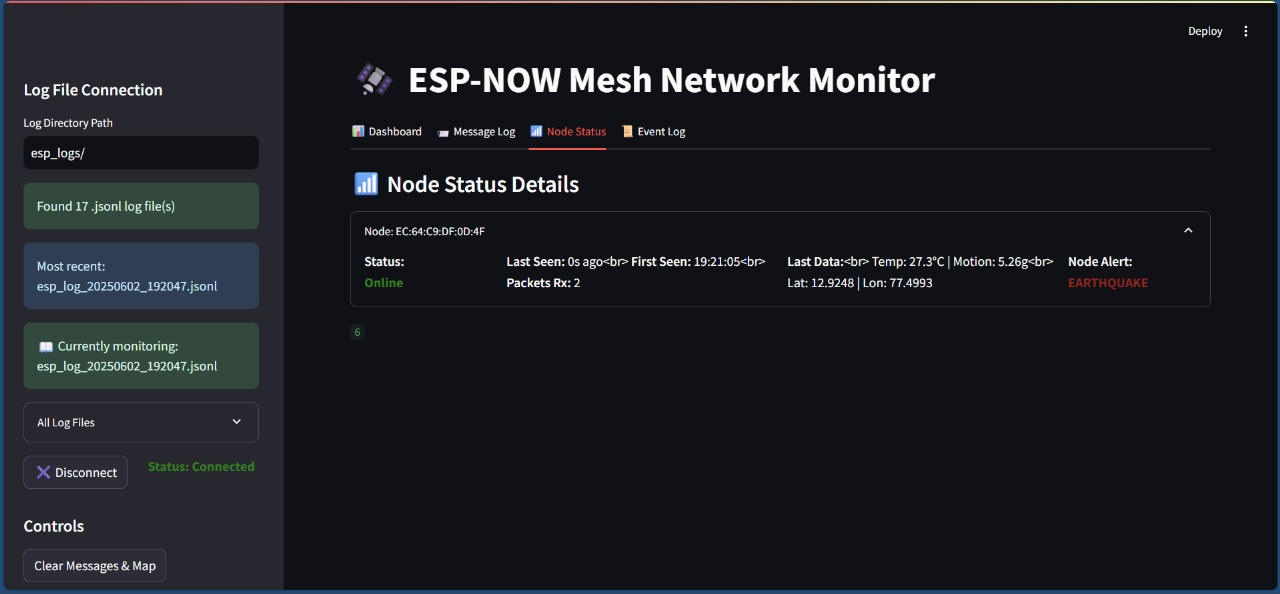
\includegraphics[width=0.8\textwidth]{prototype2.jpg} % Placeholder for your mobile gateway photo
    \caption{Mobile Gateway (e.g., on a drone or vehicle mockup)}
    \label{fig:prototype_2}
\end{figure}

\begin{figure}[H]
    \centering
    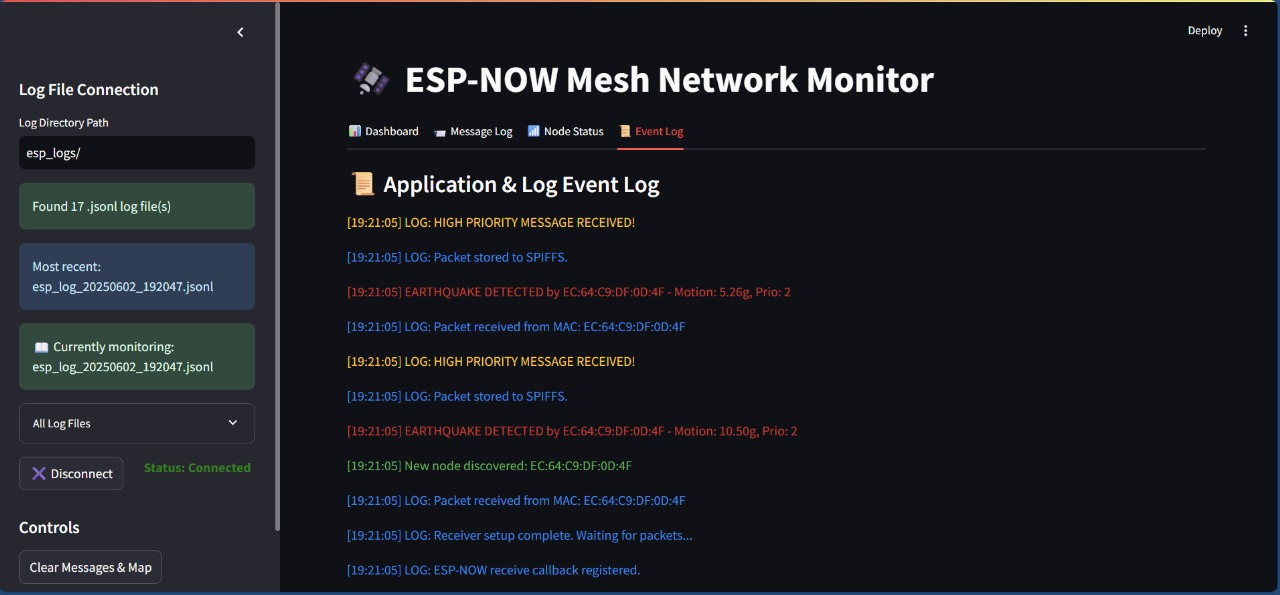
\includegraphics[width=0.8\textwidth]{prototype3.jpg} % Placeholder for communication test results (e.g., serial monitor output)
    \caption{Screenshot of Message Flow (e.g., Serial Monitor Output)}
    \label{fig:message_flow}
\end{figure}

\textit{Further results will include:}
\begin{itemize}
    \item Screenshots of the base station interface displaying received messages.
    \item Log data showing message delivery success rates under various simulated disaster conditions.
    \item Power consumption analysis for different node roles.
\end{itemize}
This framework holds significant promise for enhancing communication resilience in the face of disasters, providing a vital tool for humanitarian efforts and emergency response.

\clearpage
% --- References (Optional, but good practice) ---
\section{References}
\begin{thebibliography}{99}
    \bibitem{ESP32_Datasheet} Espressif Systems. (2017). \textit{ESP-WROOM-32 Datasheet (V2.1)}.
    \bibitem{ESPNOW_Docs} Espressif Systems. (n.d.). \textit{ESP-NOW - Arduino ESP32 latest documentation}.
    \bibitem{MPU6050_Datasheet} InvenSense. (n.d.). \textit{MPU-6050 Datasheet}. All About Circuits.
    \bibitem{NEO6M_Datasheet} U-blox. (n.d.). \textit{U-blox NEO-6M Datasheet}. Techtonics.
    \bibitem{MQ2_Datasheet} Hanwei Electronics Co., Ltd. (n.d.). \textit{MQ-2 Gas Sensor Datasheet}. Components101.
    \bibitem{DHT22_Datasheet} Aosong Electronics Co.,Ltd. (n.d.). \textit{DHT22 Digital-output relative humidity \& temperature sensor/module Datasheet}. Alldatasheet.com.
    \bibitem{Hassan2017} Hassan, S. A., Ahmed, R., \& Khan, A. (2017). \textit{Internet of Things for Disaster Management: State-of-the-Art and Prospects}. IEEE Access.
    \bibitem{Bellido2023} Bellido, F. J., López-García, G., \& Sánchez-Maestre, M. P. (2023). \textit{Emergency Communication System Based on Wireless LPWAN and SD-WAN Technologies: A Hybrid Approach}. Electronics (MDPI).
    \bibitem{Diaz2012} Diaz, C. A., Barrantes, A., \& Sanchez, J. G. (2012). \textit{Evaluating Opportunistic Networks in Disaster Scenarios}. ResearchGate.
    \bibitem{Khan2022} Khan, A. U., Khan, M. E., Hasan, M., Zakri, W., Alhazmi, W., & Islam, T. (2022). \textit{An Efficient Wireless Sensor Network Based on the ESP-MESH Protocol for Indoor and Outdoor Air Quality Monitoring}. Sustainability (MDPI).
\end{thebibliography}

\end{document}